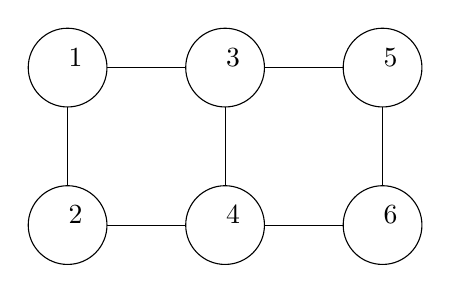
\begin{tikzpicture}
  %ノード1  
  \draw(4,2) circle (0.5)
  node[at={(4.1,2.1)}] {
    \begin{tabular}{c}
      1
    \end{tabular}
  };
  %ノード2  
  \draw(4,0) circle (0.5)
  node[at={(4.1,0.1)}] {
    \begin{tabular}{c}
      2
    \end{tabular}
  };
  %ノード3  
  \draw(6,2) circle (0.5)
  node[at={(6.1,2.1)}] {
    \begin{tabular}{c}
      3
    \end{tabular}
  };
  %ノード4  
  \draw(6,0) circle (0.5)
  node[at={(6.1,0.1)}] {
    \begin{tabular}{c}
      4
    \end{tabular}
  };
  %ノード5  
  \draw(8,2) circle (0.5)
  node[at={(8.1,2.1)}] {
    \begin{tabular}{c}
      5
    \end{tabular}
  };
  %ノード6  
  \draw(8,0) circle (0.5)
  node[at={(8.1,0.1)}] {
    \begin{tabular}{c}
      6
    \end{tabular}
  };
\draw(4,0.5) --(4,1.5);
\draw(6,0.5) --(6,1.5);
\draw(8,0.5) --(8,1.5);
\draw(4.5,0) --(5.5,0);
\draw(4.5,2) --(5.5,2);
\draw(6.5,0) --(7.5,0);
\draw(6.5,2) --(7.5,2);
\end{tikzpicture}
